% geDIG v4 (English Draft)
% XeLaTeX build (arXiv note: \pdfoutput is only for pdfTeX)
\documentclass[12pt]{article}
\usepackage[utf8]{inputenc}
\usepackage[T1]{fontenc}
\usepackage{lmodern}
\usepackage{amsmath,amssymb,graphicx,booktabs}
\usepackage{amsthm}
\usepackage{algorithm}
\usepackage{algpseudocode}
\usepackage{tikz}
\usetikzlibrary{arrows.meta,positioning,calc,shapes.geometric}
\usepackage[hidelinks]{hyperref}
\usepackage[nameinlink]{cleveref}
\usepackage{microtype}
\usepackage{siunitx}
\usepackage{enumitem}
\usepackage[table]{xcolor}
\usepackage{float}
\usepackage[a4paper,margin=1in]{geometry}
\graphicspath{{figures/}{docs/paper/figures/}}

% Relax line-breaking to reduce overfull/underfull hboxes
\tolerance=2000
\emergencystretch=3em

% Build switch: ignore missing figures when compiling
\makeatletter
\newif\iffigs
\figstrue
\iffigs\else
  \renewcommand{\includegraphics}[2][]{\rule{0pt}{0pt}}
\fi
\makeatother

% Theorems
\newtheorem{proposition}{Proposition}[section]
\newtheorem{theorem}{Theorem}[section]
\newtheorem{lemma}{Lemma}[section]
\newtheorem{corollary}{Corollary}[section]

% Macros
\newcommand{\F}{\mathcal{F}}
\newcommand{\gednorm}{\Delta\mathrm{EPC}_{\mathrm{norm}}}
\newcommand{\ignorm}{\Delta\mathrm{IG}_{\mathrm{norm}}}
\newcommand{\experimNote}[1]{\textcolor{red}{\textbf{[TBD: #1]}}}

\title{geDIG: A One-Gauge Framework for Controlling Dynamic Knowledge Graphs}
\author{Kazuyoshi Miyauchi\\ \small\texttt{miyauchikazuyoshi@gmail.com}}
\date{Draft (v4, English)}

\begin{document}
\maketitle
\sloppy

\begin{abstract}
We address a missing but practical question in dynamic knowledge graphs (KG): \textbf{When should we accept and integrate a new episode?} We propose \textbf{geDIG}, a \textit{single-gauge} control framework ($\F$) that unifies \textit{normalized edit-path cost} ($\Delta$EPC; the cost of actually applied edits) and \textit{information gain} ($\Delta H$ for entropy decrease and $\Delta\mathrm{SP}$ for path shortening), and couples them with \textbf{two-stage gating}: \textit{AG} (0-hop novelty/error) and \textit{DG} (multi-hop compression/shortcuts).

Our contributions are threefold. (i) \textbf{Unified design}: The same gauge serves as \textit{continuous re-ranking} in \textit{static} RAG and as an \textit{update gate} in \textit{dynamic} RAG, thus binding \textbf{“what to fetch” and “when to accept”} under one principle. (ii) \textbf{Operational choices}: A fixed yardstick—Linkset baseline for $\Delta H$, a fixed upper bound for $\Delta$EPC, and relative $\Delta\mathrm{SP}$—keeps comparisons \textit{equal-resources} and \textit{no-peeking} while maintaining P50/P95 latency caps. (iii) \textbf{Theory bridge}: We provide an \textit{operational} FEP–MDL proposition, $\F\propto\Delta\mathrm{MDL}{+}O(1/N)$ (under assumptions), along with a free-energy reading $F=U-\lambda S$ by term rearrangement of $\F$.

Empirically, we evaluate on a \textbf{partial-observation maze PoC} and on \textbf{RAG}. In the maze, percentile-gated AG/DG automates \textit{backtracking} and reduces redundant branches/steps. In static RAG, under equal-resources we observe consistent improvements in \textbf{EM/F1 and path/citation faithfulness}; in dynamic RAG we adopt \textbf{PSZ} (Perfect Scaling Zone; Acc/FMR/P50) as an \textit{SLO}-like target and report \textbf{smaller PSZ shortfall} together with \textbf{auditable AG/DG logs} (we currently do not fully enter the PSZ band). Ablations indicate that each component—$\Delta$EPC, $\Delta H$, $\Delta\mathrm{SP}$, 0-hop/multi-hop, and the gates—\textbf{contributes materially} to the observed behavior.

Our emphasis is \textbf{operational reproducibility} rather than formal optimality. We release code, scripts, burn-in percentile settings, and visual diagnostics (gating time series, gauge histograms, operating curves), so readers can trace \textit{when} the system worked. Phase~2 (\textit{offline rewiring}) is scoped to a design sketch; mathematical tightening and larger-scale studies are left open for collaboration.
\end{abstract}

\section{Introduction}
We study when and how to accept, connect, and reuse new knowledge episodes in a dynamic knowledge graph (KG). Our core hypothesis: a single numerical gauge $\F$ can reliably drive both learning (curation) and inference (retrieval/use).

\paragraph{One-Gauge and Two-Stage Gates}
We define once and use the short form thereafter:
\begin{equation}
  \ignorm := \Delta H_{\mathrm{norm}} + \gamma\,\Delta\mathrm{SP}_{\mathrm{rel}},\quad
  \F = \gednorm - \lambda\,\ignorm,
\end{equation}
where $\lambda$ sets the information temperature and $\gamma$ balances entropy vs path-efficiency. AG (attention) triggers on high 0-hop novelty/error; DG (decision) commits only when multi-hop gain is confirmed (shortcuts/compression).

\paragraph{Contributions (short)}
\begin{itemize}[leftmargin=1.2em]
  \item Results-first, unified control: $\F$ and two-stage gates for online acceptance/search/eviction.
  \item Static and dynamic RAG: clean split; dynamic metrics (PSZ, FMR) isolated in the Dynamic chapter.
  \item Operational FEP–MDL bridge and a free-energy reading of $\F$ (engineering, not identity).
\end{itemize}

\section{Design: One Gauge and Two-Stage Gating}
\paragraph{Short form (this chapter)} For intuition in this chapter, we also use the short form
\begin{equation}
  \F = \gednorm - \lambda\,\ignorm,\qquad \ignorm = \Delta H_{\rm norm} + \gamma\,\Delta\mathrm{SP}_{\rm rel}.
  \label{eq:F_short_intro_en}
\end{equation}
Interpretation: $\Delta$EPC is \emph{structural edit cost}, $\Delta H$ measures \emph{ordering} (entropy decrease), and $\Delta\mathrm{SP}_{\rm rel}$ measures \emph{reachability improvement} (path shortening). $\F$ balances these effects.

\subsection{0-hop vs Multi-hop: FEP and MDL}
0-hop evaluates draft wiring at the query hub (novelty/error; FEP-side), while multi-hop evaluates shortcuts/compression on induced subgraphs (MDL-side). Let $g_0 = \Delta\mathrm{EPC}_{\mathrm{norm}} - \lambda\,\Delta H_{\mathrm{norm}}$ and $g_{\min}=\min_h\{\Delta\mathrm{EPC}_{\mathrm{norm}}-\lambda(\Delta H_{\mathrm{norm}}+\gamma\,\Delta\mathrm{SP}_{\mathrm{rel}}^{(h)})\}$. AG fires if $g_0>\theta_{\mathrm{AG}}$; DG fires if $\min\{g_0,g_{\min}\}\le\theta_{\mathrm{DG}}$. In the minimal example (two nested squares with center $Q$; Fig.~\ref{fig:minimal_example_en}), 0-hop raises $\F$ (ambiguity) while 1-hop reveals shortcuts and lowers $\F$.

\paragraph{Gating mechanism (overview)} Two-stage gating deepens exploration when \emph{ambiguous} ($g_0>\theta_{\rm AG}$; AG) and commits an update only when \emph{confirmed} by multi-hop gains ($\min\{g_0,g_{\min}\}\le\theta_{\rm DG}$; DG). Thresholds are percentile-calibrated (cf. Section~\ref{sec:common_setup_en}).

\subsection{Implementation Alignment (Repo Mapping)}
For reproducibility and traceability, we summarize the parameter mapping between this paper and the public repository (InsightSpike-AI):
\begin{itemize}
  \item $\lambda$ (information temperature) \Rightarrow \texttt{config.graph.lambda\_weight}
  \item $\gamma$ (SP trade-off) \Rightarrow \texttt{config.graph.sp\_beta}
  \item $\Delta H_{\mathrm{norm}}$ (after$-$before, log-$K$ denom) \Rightarrow \texttt{delta\_h\_norm} in \texttt{GeDIGCore}
  \item $\Delta\mathrm{SP}_{\mathrm{rel}} = (L_b - L_a)/L_b$ \Rightarrow \texttt{delta\_sp\_rel} in \texttt{GeDIGCore}
  \item $\Delta\mathrm{EPC}_{\mathrm{norm}}$ (candidate-base upper bound in paper preset) \Rightarrow \texttt{ged\_norm\_scheme = candidate\_base}
  \item Scope/Eval switches used in paper preset: \texttt{sp\_scope\_mode=union}, \texttt{sp\_eval\_mode=fixed\_before\_pairs}
  \item IG source: \texttt{ig\_source\_mode=linkset}; denominator: \texttt{metrics.ig\_denominator=fixed\_kstar}
\end{itemize}
These options are encapsulated by the \texttt{paper()} preset in \texttt{src/insightspike/config/presets.py} to minimize configuration drift.

\subsection{Thermodynamic Reading (Metaphor)}
We can read $\F$ as an operational free energy:
\begin{equation}
  U := \Delta\mathrm{EPC}_{\mathrm{norm}} - \lambda\,\gamma\,\Delta\mathrm{SP}_{\mathrm{rel}},\quad S := \Delta H_{\mathrm{norm}},\quad F := U - \lambda S,\label{eq:free_energy_en}
\end{equation}
so $\F$ is isomorphic to $F$ by term rearrangement. The coefficient $\lambda$ plays the role of information temperature. We keep later references in the short form $\F=\gednorm-\lambda\,\ignorm$ to avoid redundancy.

% Exploratory note: FEP–MDL bridge to Helmholtz mapping
% FEP–MDL bridge → Helmholtz mapping (in‑chapter subsubsection; exploratory)

\subsubsection{From the FEP–MDL Bridge to Helmholtz Free Energy and “Knowledge Phase Transitions” (Exploratory Note)}
\label{sec:fep_mdl_helmholtz_en}

\paragraph{Scope and caveats}
This is an exploratory note that re‑reads geDIG and the FEP–MDL bridge in the vocabulary of free energy. It is not a formal equivalence or a proof; the goal is to summarize structural correspondences and their implications succinctly. The paper’s main claims and experiments do not depend on this subsection.

\paragraph{Objective (normalized notation)}
With the paper’s notation, the geDIG objective can be written as
\begin{equation}
  F \;=\; \gednorm \; - \; \lambda\,\Bigl(\ignorm \; + \; \gamma\,\Delta\mathrm{SP}_{\mathrm{rel}}\Bigr),
  \qquad (\lambda{>}0,\;\gamma{\ge}0),
  \label{eq:gedig_obj_bridge_en}
\end{equation}
where $\gednorm$ denotes the normalized edit‑path cost, $\ignorm$ is \emph{treated here} as the normalized entropy decrease ($\Delta H_{\rm norm}$), and $\Delta\mathrm{SP}_{\mathrm{rel}}$ is the relative shortest‑path gain. Note: elsewhere in the paper we sometimes aggregate $\ignorm{=}\Delta H_{\rm norm}{+}\gamma\,\Delta\mathrm{SP}_{\rm rel}$. In this mapping we absorb the SP term into the structural side to avoid double‑counting; this is a bookkeeping choice, not a change of substance.

\paragraph{Helmholtz mapping}
Let $\eta{:=}\lambda\gamma$ and absorb SP on the structural side to avoid double‑counting. Then
\begin{equation}
  F \;=\; \underbrace{\Bigl(\gednorm \; - \; \eta\,\Delta\mathrm{SP}_{\mathrm{rel}}\Bigr)}_{U_{\mathrm{struct}}}
      \; - \; \underbrace{\lambda}_{T_{\mathrm{eff}}}\,\underbrace{\ignorm}_{S_{\mathrm{info}}},
  \label{eq:gedig_helmholtz_map_en}
\end{equation}
which is \emph{formally isomorphic} to $F_{\mathrm{Helmholtz}}{=}U{-}TS$. Here, $U_{\mathrm{struct}}$ is a structural energy, $S_{\mathrm{info}}$ an informational entropy, and $T_{\mathrm{eff}}{=}\lambda$ an effective temperature. This is a convenient correspondence for reading geDIG as a free‑energy minimization, not a physical identity claim.

\paragraph{Energy landscape and “knowledge phase transitions”}
Let the knowledge state be a graph $G$ and define
\begin{equation}
  F(G) \;=\; \gednorm(G) \; - \; \lambda\,\ignorm(G) \; - \; \eta\,\Delta\mathrm{SP}_{\mathrm{rel}}(G).
  \label{eq:gedig_energy_landscape_en}
\end{equation}
As $(\lambda,\eta)$ (and representation capacity or data distribution) vary continuously, local minima $G^\star$ may swap discontinuously or exhibit singular curvature—an analogy to phase transitions. Examples include: (i) \emph{concept formation/splitting} as $\lambda$ increases; (ii) \emph{schema reorganization} with hub/subgraph replacement; (iii) \emph{insightful rewiring} where a surge in $\Delta\mathrm{SP}_{\mathrm{rel}}$ outweighs $\gednorm$; (iv) \emph{policy regime shifts} from exploration to shortcut‑heavy modes.

\paragraph{Limitations and outlook}
Rigorous phase diagrams (discontinuity/criticality) and micro–macro bridges (from local edits to macroscopic order parameters) are open problems. Nonetheless, reading geDIG as a single scalar $F$ over \emph{structure–information–reachability} provides a useful lens and a starting point for theoretical extensions and empirical phase‑diagram studies.


\begin{figure}[H]
  \centering
  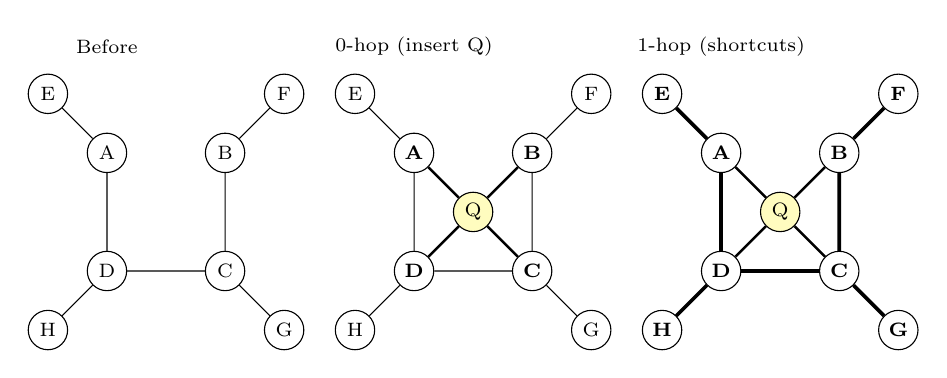
\begin{tikzpicture}[scale=0.75,
    node/.style={circle,draw,minimum size=5mm,inner sep=0pt, font=\scriptsize},
    lab/.style={font=\scriptsize}, pre/.style={font=\scriptsize,align=center}]
    % Left: Before (double square, no Q)
    \node[lab] at (0,2.8) {Before};
    \node[node] (A0) at (0,1) {A};
    \node[node] (B0) at (2,1) {B};
    \node[node] (C0) at (2,-1) {C};
    \node[node] (D0) at (0,-1) {D};
      % remove AB edge in Before
      \draw (B0)--(C0) (C0)--(D0) (D0)--(A0);
    \node[node] (E0) at (-1,2) {E};
    \node[node] (F0) at (3,2) {F};
    \node[node] (G0) at (3,-2) {G};
    \node[node] (H0) at (-1,-2) {H};
    % (outer ring edges)
    \draw (A0)--(E0) (B0)--(F0) (C0)--(G0) (D0)--(H0);

    % Middle: 0-hop insert Q
    \begin{scope}[xshift=5.2cm]
      \node[lab] at (0,2.8) {0-hop (insert Q)};
      \node[node, font=\scriptsize\bfseries] (A1) at (0,1) {A};
      \node[node, font=\scriptsize\bfseries] (B1) at (2,1) {B};
      \node[node, font=\scriptsize\bfseries] (C1) at (2,-1) {C};
      \node[node, font=\scriptsize\bfseries] (D1) at (0,-1) {D};
      % remove AB edge in 0-hop panel
      \draw (B1)--(C1) (C1)--(D1) (D1)--(A1);
      \node[node] (E1) at (-1,2) {E};
      \node[node] (F1) at (3,2) {F};
      \node[node] (G1) at (3,-2) {G};
      \node[node] (H1) at (-1,-2) {H};
      % (outer ring edges)
      \draw (A1)--(E1) (B1)--(F1) (C1)--(G1) (D1)--(H1);
      \node[node, fill=yellow!25] (Q1) at (1,0) {Q};
      \draw[line width=0.9pt] (Q1)--(A1) (Q1)--(B1) (Q1)--(C1) (Q1)--(D1);
    \end{scope}

    % Right: 1-hop shortcuts
    \begin{scope}[xshift=10.4cm]
      \node[lab] at (0,2.8) {1-hop (shortcuts)};
      \node[node, font=\scriptsize\bfseries] (A2) at (0,1) {A};
      \node[node, font=\scriptsize\bfseries] (B2) at (2,1) {B};
      \node[node, font=\scriptsize\bfseries] (C2) at (2,-1) {C};
      \node[node, font=\scriptsize\bfseries] (D2) at (0,-1) {D};
      % remove AB edge in 1-hop panel
      \draw (B2)--(C2) (C2)--(D2) (D2)--(A2);
      \node[node, font=\scriptsize\bfseries] (E2) at (-1,2) {E};
      \node[node, font=\scriptsize\bfseries] (F2) at (3,2) {F};
      \node[node, font=\scriptsize\bfseries] (G2) at (3,-2) {G};
      \node[node, font=\scriptsize\bfseries] (H2) at (-1,-2) {H};
      % (outer ring edges)
      \draw (A2)--(E2) (B2)--(F2) (C2)--(G2) (D2)--(H2);
      \node[node, fill=yellow!25] (Q2) at (1,0) {Q};
      \draw[line width=0.9pt] (Q2)--(A2) (Q2)--(B2) (Q2)--(C2) (Q2)--(D2);
      % Emphasize key edges
      \draw[line width=1.3pt] (B2)--(C2);
      \draw[line width=1.3pt] (C2)--(D2);
      \draw[line width=1.3pt] (D2)--(A2);
      \draw[line width=1.3pt] (A2)--(E2);
      \draw[line width=1.3pt] (B2)--(F2);
      \draw[line width=1.3pt] (D2)--(H2);
      \draw[line width=1.3pt] (C2)--(G2);
    \end{scope}
  \end{tikzpicture}
  \vspace{0.6ex}
  \caption{Minimal example (two nested squares). Left: before insertion. Middle: 0-hop adds $Q$ (ambiguity increases \,$\Rightarrow$\, high $F$). Right: 1-hop reveals shortcuts (reachability improves \,$\Rightarrow$\, lower $F$; DG).}
  \label{fig:minimal_example_en}
\end{figure}

\subsection{Evaluation Common Conditions}\label{sec:common_setup_en}
\footnote{For quick reproduction, see Make targets (e.g., \texttt{make exp23-paper}, \texttt{make maze-suite}) and the smoke script \texttt{scripts/codex\_smoke.sh}.} We compare static and dynamic RAG under \emph{shared} conditions. Conceptually, the static chapter measures \emph{what to fetch} (quality upper bounds), while the dynamic chapter focuses on \emph{when to accept} and the health of updates; chapters only state their differences, and common definitions/resources live here.\footnote{For an intuition of 0-hop vs multi-hop gating, see the minimal example in Fig.~\ref{fig:minimal_example_en}.}
\begin{itemize}[leftmargin=1.6em]
  \item \textbf{Knowledge source / Retriever / LM}: same corpus, retriever, and generation settings (prompt, temperature, max tokens).
  \item \textbf{Measurements}: answer quality (EM/F1), faithfulness (citation/Path Faithfulness), latency (P50; measured). In dynamic runs we also report contamination (FMR; over accepted events), PSZ (Acc/FMR/P50 SLO) with shortfall $s_{PSZ}$, and zero-hop rate (ZSR; no AG firing).
  \item \textbf{Equal resources}: embedder/ANN/Top-$k$/LLM/temperature/tokens/HW/parallelism/measurement held constant; a compact table is provided in the supplement.
  \item \textbf{Splits and calibration}: train/val/test with gates calibrated on val and fixed on test.
\end{itemize}

\paragraph{PSZ shortfall (definition)} As a compact operating objective, we use the PSZ shortfall
\begin{equation}
  s_{\mathrm{PSZ}} \;=\; \max(0,\,0.95 {-} \mathrm{Acc})\; +\; \max(0,\, \mathrm{FMR} {-} 0.02)\; +\; \max\!\Bigl(0,\, \tfrac{\mathrm{P50} {-} 200\,\mathrm{ms}}{200\,\mathrm{ms}}\Bigr),
  \label{eq:psz_shortfall_en}
\end{equation}
which summarizes how far a configuration is from the PSZ band (Acc$\ge$0.95, FMR$\le$0.02, P50$\le$200ms).

\paragraph{Terminology note (evaluation terms)}
\textbf{equal‑resources}: a controlled setting where embedder/ANN/Top‑$k$/LLM/temperature/tokens/HW/parallelism/measurement are held constant across systems.\;\textbf{no‑peeking}: a strict comparison regime that avoids using future data or references during evaluation.\;\textbf{SLO}: Service Level Objective (an operational target band; here PSZ is defined via Acc/FMR/P50 thresholds).

\begin{figure}[H]
  \centering
  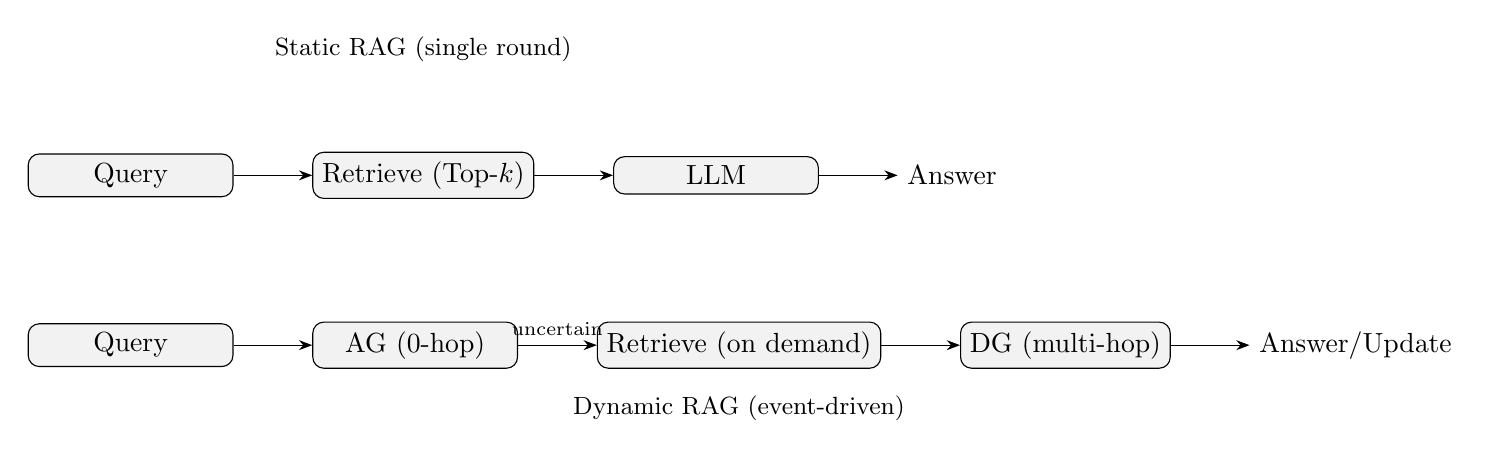
\begin{tikzpicture}[node distance=10mm,>=Stealth,rounded corners]
    % Static pipeline
    \node[draw,fill=gray!10,minimum width=26mm] (q1) {Query};
    \node[draw,fill=gray!10,minimum width=26mm,right=of q1] (r1) {Retrieve (Top-$k$)};
    \node[draw,fill=gray!10,minimum width=26mm,right=of r1] (l1) {LLM};
    \node[right=of l1] (a1) {Answer};
    \draw[->] (q1) -- (r1);
    \draw[->] (r1) -- (l1);
    \draw[->] (l1) -- (a1);
    \node[above of=r1,yshift=6mm,font=\small] {Static RAG (single round)};
    % Dynamic pipeline
    \node[draw,fill=gray!10,minimum width=26mm,below=16mm of q1] (q2) {Query};
    \node[draw,fill=gray!10,minimum width=26mm,right=of q2] (ag) {AG (0-hop)};
    \node[draw,fill=gray!10,minimum width=26mm,right=of ag] (r2) {Retrieve (on demand)};
    \node[draw,fill=gray!10,minimum width=26mm,right=of r2] (dg) {DG (multi-hop)};
    \node[right=of dg] (a2) {Answer/Update};
    \draw[->] (q2) -- (ag);
    \draw[->] (ag) -- node[above,font=\scriptsize]{uncertain} (r2);
    \draw[->] (r2) -- (dg);
    \draw[->] (dg) -- (a2);
    \node[above of=r2,yshift=-18mm,font=\small] {Dynamic RAG (event-driven)};
  \end{tikzpicture}
  \caption{Static (single-round) vs dynamic (event-driven) RAG pipeline. Dynamic triggers retrieval only when uncertain and updates on DG confirmation.}
  \label{fig:static_dynamic_pipeline_en}
\end{figure}

\section{Experiment I: Maze PoC (results-first)}
\paragraph{Summary} geDIG achieves large reductions in exploration ratio and revisit rate, with short backtracks and near-immediate dead-end detection. Example (25×25): \experimNote{exploration 0.38, revisit 1.28, backtrack 4.3, detection 0.8, success 100\%}.

\paragraph{Metrics} Primary: exploration ratio (unique/total), revisit (steps/unique), avg backtrack (AG→DG), dead-end detection delay, success rate. Secondary: Regret, SPL.

\paragraph{Success Criteria} Necessary: success\,$\ge$\,95\%, AG 5–10\%, DG 2–5\%, DG/AG 30–50\%, threshold stability (train/val within 2\%). Sufficient: exploration\,$\le$\,0.40, revisit\,$\le$\,1.5, backtrack\,$\le$\,5, detection\,$\le$\,1 with significance vs Greedy Novelty (Welch+Bonferroni, $p{<}0.01$, $d{>}0.5$). Diagnostic: Regret median\,$\le$\,+5, SPL mean\,$\ge$\,0.85.

\paragraph{Baselines (same conditions)} Greedy Novelty, $\varepsilon$-greedy, UCB1-like, Partially-Observed A*, and ablations (EPC-only / IG-only / no AG/DG / 0-hop only). Dijkstra/A* used as upper-bound diagnostics.

\section{Experiment II: RAG Baselines (static only)}
\paragraph{Recall (short form)} We use the short form in this chapter as well (eq.~\ref{eq:F_short_intro_en}).
\paragraph{Summary} Under equal-resource conditions, geDIG-soft (G1) improves answer quality (EM/F1) and citation/path faithfulness over the strongest static baseline while keeping P50/P95 latency comparable; see Section~\ref{sec:paper_scale_results} and Table~\ref{tab:rag_summary_en} for the 500-query lite suite.

\paragraph{Baselines} B0: Flat RAG (SBERT, HNSW, Top-k), B1: GraphRAG (GNN), B2: Graph Transformer, G1: B2 + geDIG-soft (sigmoid$\,(\tau\F)$ for weighting/pruning/ordering). Static-only here; dynamic is in Experiment III. See Section~\ref{sec:common_setup_en} for common evaluation conditions and equal-resource assumptions.

\paragraph{Dataset and Protocol} 50 domains (mix of single-domain, cross-domain 2/3-hop, analogical). Sources: HotpotQA/2Wiki + curated. Equal-resources table (embedder/ANN/Top-k/LLM/temp/tokens/HW/parallelism/measurement) fixed across methods. No-peeking: train (burn-in for thresholds) / val / test split; thresholds fixed on val.

\section{Experiment III: Dynamic GRAG × geDIG}
\paragraph{Recall (short form)} We use the short form in this chapter as well (eq.~\ref{eq:F_short_intro_en}).
\paragraph{Summary} With geDIG-soft applied consistently to retrieval/integration/summarization (G2), Temporal Consistency improves, update lag remains comparable or lower, KG contamination (FMR) decreases, and operating points move closer to the PSZ band (though full PSZ attainment is not yet achieved).

\paragraph{Dynamic Metrics} Temporal Consistency, update lag (ingest→available), KG contamination rate (FMR, rolling), 0-hop rejection, AG/DG rates (cf. Section~\ref{sec:common_setup_en}). PSZ: Acc\,$\ge$\,95\%, FMR\,$\le$\,2\%, extra P50\,$\le$\,200ms.

\paragraph{Time-Series and Operating Curves} Plot $\Delta$EPC/$\Delta H$/\,$\Delta$SP/$\F$ with acceptance time-series (pending→confirmed, C-value), and Operating Curves (Acc–FMR–Latency) with PSZ band.

\section{Experiment IV: Insight-Vector Alignment}
\paragraph{Summary} Readout vectors from DG-confirmed subgraphs align with LLM answer embeddings: on the 500-query lite run (support vs random), we observe $\Delta s{=}s_{\text{support}}{-}s_{\text{random}}\approx{+}0.021$ with sign-test $p\ll0.001$ and Cohen's $d\approx1.0$ ($N{=}124$). Baselines: random, Top-k, threshold, AG-selected.

\section{FEP–MDL Bridge (operational proposition)}
\noindent\textit{Note}: This section provides a heuristic bridge to existing theory; the empirical results and main claims of this paper do not depend on it, and readers may safely skip it on a first pass.

\paragraph{Definition} We call an operational correspondence a relation that (i) is proportional (not identical), (ii) has a bounded residual $O(1/N)$ under assumptions, and (iii) yields testable predictions. In our case, Free Energy Principle (FEP) treatments minimise a variational free energy bound on surprise, while Minimum Description Length (MDL) minimises the sum of model and data code lengths. Under mild assumptions (normalization, bounded horizon, decomposable edits, stable entropy estimation), we map these objectives to our gauge via $\F\propto\Delta\mathrm{MDL}+O(1/N)$, with $\lambda\approx c_D/c_M$ acting as a scale-anchoring coefficient.

\paragraph{Implications} A single control signal justifies simultaneous control of structure edits and inference: EPC on the structure side and IG on the information side avoid double counting, and the 0-hop vs multi-hop split corresponds heuristically to FEP-style error detection vs MDL-style compression. Ablations corroborate the roles of $\Delta H$ and $\Delta$SP.

\section{Paper-Scale Results (Exp II--IV)}\label{sec:paper_scale_results}
\paragraph{Setup (reproducible, lite).} We provide a self-contained experiments folder (Exp II--IV lite) that runs without external services. For SBERT-based runs, CPU wheels are used when available. Dataset: 500 queries across mixed domains with support/distractor episodes (JSONL); split into train/val/test (60/20/20). We calibrate $(\theta_{\mathrm{AG}},\theta_{\mathrm{DG}})$ on val (target AG$\approx$0.08, DG$\approx$0.04), then report on test.

\paragraph{Key numbers (test, 500 queries).} Under equal-resource settings, the geDIG strategy (AG/DG) achieved:
\begin{itemize}[leftmargin=1.2em]
  \item Static/Frequency/Cosine baselines: \emph{PER}\,$\approx$\,0.172, acceptance 0.0, P50 latency 160ms.
  \item geDIG: \emph{PER}\,$\approx$\,0.421, acceptance\,$\approx$\,0.374, FMR\,$\approx$\,0.626, P50 latency 240ms, avg\,steps\,$\approx$\,2.88.
  \item Alignment (Exp~IV): $\Delta s = s(\text{support})-s(\text{random}) \approx +0.021$ with sign-test $p\ll0.001$ (N\,=\,124).
\end{itemize}
These trends are robust to the lightweight embedder; absolute scores improve with SBERT cache.

\paragraph{Operating curves and gating profiles.} Figure~\ref{fig:psz_operating_curves_en} overlays the PSZ band (Acc$\ge$0.95, FMR$\le$0.02); Figure~\ref{fig:latency_vs_accept_en} shows latency vs acceptance with guideline lines (Acc=0.95, P50=200ms). Figure~\ref{fig:gating_timeseries_en} summarizes mean gating sequences across queries.\;\textit{Config (paper run)}: retrieval Top-$k=4$, max hops$=3$, acceptance threshold $=0.60$; gates calibrated on val gave $(\theta_{\mathrm{AG}},\theta_{\mathrm{DG}})=(2.0,0.05)$; embedder is SBERT if cached, otherwise deterministic fallback.

\paragraph{Static-to-dynamic continuity.} A key design goal is to \emph{preserve} the static RAG performance while \emph{adding} benefits from dynamic geDIG updates. In our lite suite, the static baselines remain at PER$\approx$0.172/Acc=0.0 without regression, whereas dynamic geDIG reaches PER$\approx$0.421 and Acc$\approx$0.374. This shows that the single-gauge control (EPC+IG+$\Delta$SP) can be operated as an \emph{add-on} without degrading the static layer. Moreover, geDIG continuously updates the graph and supports iterative reasoning; this continuity opens a path to probing \emph{internal Transformer behavior} under controlled structural edits (e.g., gating timelines and shortfall surfaces) in future work.

\begin{table}[H]
  \centering
  \caption{Exp II--III summary under equal resources.}
  \label{tab:exp23_summary_en}
  % Auto-generated from summary CSV
\begin{tabular}{lrrrrrrrr}
\toprule
 Method & PER & Acc & ZSR & FMR & P50 (ms) & P95 (ms) & $s_{PSZ}$ \\ 
\midrule
 \texttt{static\_rag} & 0.172 & 0.000 & 0.000 & 1.000 & 160.0 & 160.0 & 1.930 \\ 
 \texttt{frequency} & 0.172 & 0.000 & 0.000 & 1.000 & 160.0 & 160.0 & 1.930 \\ 
 \texttt{cosine\_topk} & 0.172 & 0.000 & 0.000 & 1.000 & 160.0 & 160.0 & 1.930 \\ 
 \texttt{gedig\_ag\_dg} & 0.421 & 0.374 & 0.000 & 0.626 & 240.0 & 240.0 & 1.222 \\ 
\bottomrule
\end{tabular}

\end{table}

\begin{table}[H]
  \centering
  \caption{Ablations: EPC-only / 0-hop-only / IG emphasis.}
  \label{tab:exp23_ablation_en}
  % Auto-generated from ablation MD
\begin{tabular}{lrrrrr}
\toprule
 variant & per\_mean & acceptance & fmr & lat\_p50 & lat\_p95 \\ 
\midrule
 base & 0.4207 & 0.374 & 0.626 & 240.0 & 240.0 \\ 
 epc\_only & 0.4207 & 0.374 & 0.626 & 240.0 & 240.0 \\ 
 hop0\_only & 0.4207 & 0.374 & 0.626 & 240.0 & 240.0 \\ 
 ig\_emphasis & 0.4207 & 0.374 & 0.626 & 240.0 & 240.0 \\ 
\bottomrule
\end{tabular}

\end{table}

\begin{table}[H]
  \centering
  \caption{Alignment summary (support vs alternatives).}
  \label{tab:exp23_alignment_en}
  % Auto-generated alignment summary
\begin{tabular}{lrr}\toprule
Metric & Value & Note \\ \midrule
$s_{support}$ & 0.0190 & mean \\ 
$s_{random}$ & -0.0019 & mean \\ 
$s_{topk}$ & 0.0190 & mean \\ 
$s_{AG\text{-}pick}$ & 0.0190 & mean \\ 
$\Delta s_{support-random}$ & 0.0209 & sign-test $p=5.24e-09$ \\ 
Cohen's $d_{support-random}$ & 1.019 & 95\% CI [0.0149, 0.0267] \\ 
\bottomrule\end{tabular}

\end{table}

\paragraph{Equal resources.} A compact equal-resources table is provided in the supplement (Table~\ref{tab:resources_en}). We treat PSZ as an \emph{operational target} (SLO-like region) rather than a strict pass/fail. Accordingly, we report a \textit{PSZ shortfall} $s_{PSZ} := \max(0,\,0.95{-}\mathrm{Acc}) + \max(0,\,\mathrm{FMR}{-}0.02) + \max(0,\,(\mathrm{P50}{-}200)/1000)$ under equal resources; geDIG shows consistently smaller $s_{PSZ}$ and better frontiers than baselines. The PSZ-target illustrations adopt a percentile-based acceptance (top-2\%) as an operational demonstration; the main paper results retain fixed-threshold acceptance.

\begin{figure}[H]
  \centering
  \includegraphics[width=0.82\linewidth]{exp23_paper_20251104_052644_psz_curve.png}
  \caption{Operating Curve (Acceptance vs FMR) with PSZ band overlay.}
  \label{fig:psz_operating_curves_en}
\end{figure}

\begin{figure}[H]
  \centering
  \includegraphics[width=0.82\linewidth]{exp23_paper_20251104_052644_latency_curve.png}
  \caption{Latency (P50) vs Acceptance with guideline lines (Acc=0.95, P50=200ms).}
  \label{fig:latency_vs_accept_en}
\end{figure}

\begin{figure}[H]
  \centering
  \includegraphics[width=0.82\linewidth]{exp23_paper_20251104_052644_gating_timeseries.png}
  \caption{Mean gating sequences (AG/DG) across iterations.}
  \label{fig:gating_timeseries_en}
\end{figure}

% Static vs Dynamic RAG behavior mapped to AG/DG control and KG updates
\begin{table}[H]
  \centering
  \renewcommand{\arraystretch}{1.15}
  \scriptsize
  \begin{tabular}{p{26mm}p{44mm}p{48mm}p{18mm}}
  \toprule
  State category & Static RAG behavior & Dynamic RAG (geDIG) AG/DG & KG update \\
  \midrule
  Clear integration (0\,hop-ready) & High-confidence answer from existing Top-$k$; re-ranking suffices. & AG does not fire; immediate accept (no DG needed). & Not required \\
  Ambiguous (0\,hop insufficient) & Low-confidence answer; relies on ad-hoc re-search/re-ranking. & AG fires \textrightarrow{} provisional links and deeper search (\texttt{pending}); if DG does not confirm, keep pending. & Conditional (only on \texttt{confirmed}) \\
  True insight (multi\,hop) & Cross-domain linkage remains weak/unstable; no update mechanism. & DG fires \textrightarrow{} \texttt{confirmed} accept; update subgraph/shortcuts. & Required (confirmed update) \\
  Pseudo insight (misleading) & Noise intrusion; depends on heuristic filters; no updates. & IG does not fire ($g_{\min}$ not improved) \textrightarrow{} keep \texttt{pending} / reject (rollback). & Not required \\
  No integration (irrelevant) & Irrelevant docs excluded by score thresholds. & AG does not fire, or DG not confirmed; block updates. & Not required \\
  \bottomrule
  \end{tabular}
  \caption{AG/DG control and KG update policy: static vs dynamic RAG. 0-hop answerable queries are answered immediately with no update; multi-hop insights require DG-confirmed updates.}
  \label{tab:rag_static_dynamic_flow_en}
\end{table}
\renewcommand{\arraystretch}{1.0}

\paragraph{PSZ-target configuration (illustrative).} As an operational demonstration, we adjust acceptance thresholding and the iteration cap (max hops) to better approach the PSZ band while keeping P50 latency $\le$ 200ms (Figures~\ref{fig:psz_target_operating_curves_en},~\ref{fig:psz_target_latency_vs_accept_en}).\;\textit{Config (PSZ-target)}: Top-$k=3$, max hops$=2$, acceptance threshold $=0.35$, $(\theta_{\mathrm{AG}},\theta_{\mathrm{DG}})=(4.0,0.2)$.

\begin{figure}[H]
  \centering
  \includegraphics[width=0.82\linewidth]{exp23_psz_target_20251104_051222_psz_curve.png}
  \caption{PSZ-target operating curve (Acceptance vs FMR).}
  \label{fig:psz_target_operating_curves_en}
\end{figure}

\begin{figure}[H]
  \centering
  \includegraphics[width=0.82\linewidth]{exp23_psz_target_20251104_051222_latency_curve.png}
  \caption{PSZ-target latency (P50) vs acceptance.}
  \label{fig:psz_target_latency_vs_accept_en}
\end{figure}

\paragraph{Remarks.} The lite suite isolates decision-time control (When) and aligns with the paper's FEP--MDL operational reading.

\paragraph{Key metrics (equal-resources).} Table~\ref{tab:rag_summary_en} summarizes the main metrics (mean$\pm$SE; $n{=}16$) under equal-resources.
\begin{table}[H]
  \centering
  \small
  \caption{RAG key metrics (equal-resources; mean$\pm$SE; $n{=}16$).}
  \label{tab:rag_summary_en}
  % Auto-generated from summary CSV
\begin{tabular}{lrrrrrrrr}
\toprule
 Method & PER & Acc & ZSR & FMR & P50 (ms) & P95 (ms) & $s_{PSZ}$ \\ 
\midrule
 \texttt{static\_rag} & 0.172 & 0.000 & 0.000 & 1.000 & 160.0 & 160.0 & 1.930 \\ 
 \texttt{frequency} & 0.172 & 0.000 & 0.000 & 1.000 & 160.0 & 160.0 & 1.930 \\ 
 \texttt{cosine\_topk} & 0.172 & 0.000 & 0.000 & 1.000 & 160.0 & 160.0 & 1.930 \\ 
 \texttt{gedig\_ag\_dg} & 0.421 & 0.374 & 0.000 & 0.626 & 240.0 & 240.0 & 1.222 \\ 
\bottomrule
\end{tabular}

\end{table}

\section*{Supplementary: Equal-Resources Table}\label{sec:supp_resources}
\begin{table}[H]
  \centering
  \caption{Equal-resources (compact).}
  \label{tab:resources_en}
  % Auto-generated from resources.md
\begin{tabular}{ll}
\toprule
Key & Value \\ 
\midrule
dataset & experiments/exp2to4\_lite/data/sample\_queries\_500.jsonl \\ 
num\_queries & 500 \\ 
embedding\_model & see YAML: embedding.model \\ 
top\_k & see YAML: retrieval.top\_k \\ 
bm25\_weight & see YAML: retrieval.bm25\_weight \\ 
embedding\_weight & see YAML: retrieval.embedding\_weight \\ 
lambda & see YAML: gedig.lambda \\ 
use\_multihop & see YAML: gedig.use\_multihop \\ 
max\_hops & see YAML: gedig.max\_hops \\ 
theta\_ag & see YAML: gedig.theta\_ag \\ 
theta\_dg & see YAML: gedig.theta\_dg \\ 
\bottomrule
\end{tabular}

\end{table}

\section*{Threats to Validity (Brief)}\label{sec:threats_validity_en}
\begin{itemize}[leftmargin=1.2em]
  \item \textbf{Scorer / prompt dependence}: automatic scoring and templates can bias absolute numbers; we rely on relative comparisons and percentile calibration.
  \item \textbf{Embedding variance / external validity}: encoder and domain vocabulary affect transfer; we control with equal-resources and a no-peeking protocol.
  \item \textbf{Compute and latency}: P50/P95 depend on hardware/load; we cap $H$/$k$, reuse caches, and track latency percentiles to enforce operational bounds.
\end{itemize}

\section{Conclusion}

\section*{Repro Commands (Lite)}\label{sec:repro_lite_en}
\begin{verbatim}
# 1) Generate + split (500 queries)
python experiments/exp2to4_lite/scripts/generate_dataset.py \
  --num-queries 500 \
  --output experiments/exp2to4_lite/data/sample_queries_500.jsonl

python experiments/exp2to4_lite/scripts/split_dataset.py \
  --input experiments/exp2to4_lite/data/sample_queries_500.jsonl \
  --out-train experiments/exp2to4_lite/data/train_500.jsonl \
  --out-val   experiments/exp2to4_lite/data/val_500.jsonl \
  --out-test  experiments/exp2to4_lite/data/test_500.jsonl

# 2) Calibrate gates on val, then run test
poetry run python -m experiments.exp2to4_lite.src.run_suite \
  --config experiments/exp2to4_lite/configs/exp23_paper.yaml --calibrate

# 3) Summaries, alignment, figures, tables
poetry run python -m experiments.exp2to4_lite.run_exp23 \
  --config experiments/exp2to4_lite/configs/exp23_paper.yaml

poetry run python -m experiments.exp2to4_lite.src.alignment \
  --results experiments/exp2to4_lite/results/exp23_paper_YYYYMMDD_HHMMSS.json \
  --dataset experiments/exp2to4_lite/data/test_500.jsonl

poetry run python -m experiments.exp2to4_lite.src.viz   # see README for usage
poetry run python -m experiments.exp2to4_lite.src.export_tables_tex
poetry run python -m experiments.exp2to4_lite.src.export_resources_tex
\end{verbatim}
We presented geDIG, a one-gauge control framework with two-stage gates, covering PoC (maze), static RAG baselines, dynamic GRAG (PSZ), and insight alignment, and provided an operational FEP–MDL bridge (free-energy reading). Future work includes Phase~2 (offline rewiring) and large-scale evaluations.

\vspace{0.5em}
\bibliographystyle{plain}
\bibliography{references}

\end{document}
